\section{\large Ejercicio 1. Conceptualización de sistemas de ecuaciones lineales en el plano.}

Dibuje una gráfica en GeoGebra que corresponda al sistema de ecuaciones lineales dado y determine geométricamente si cada sistema tiene una solución única, un número infinito de soluciones o ninguna solución. Luego, resuelva cada sistema algebraicamente para confirmar su respuesta.

\[
\begin{cases}
    \begin{aligned}
        5x+3y &=-1 \\
        -2x-5y &=5
    \end{aligned}
\end{cases}
\]

\textbf{Solución en GeoGebrara}
\begin{figure}[ht!]
    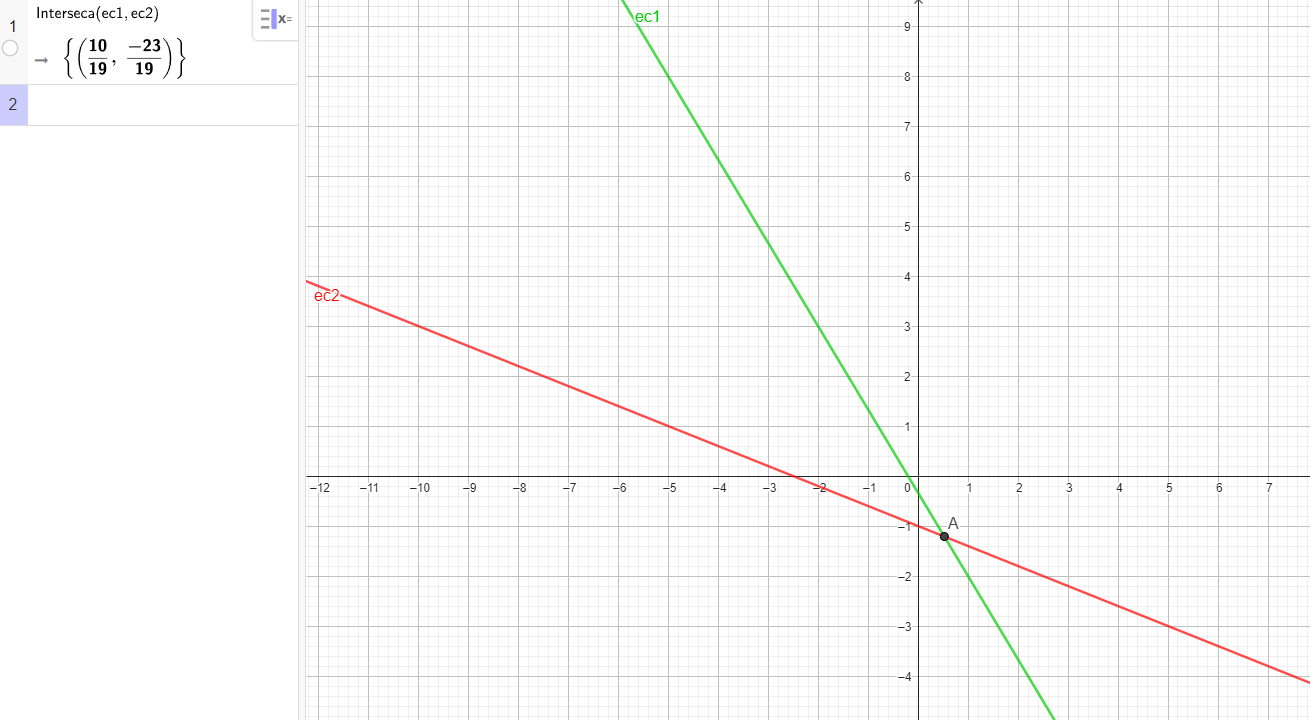
\includegraphics[width=\textwidth]{geogebra1.png}
\end{figure}

\textbf{Solución algebraica}

\begin{enumerate}
    \item Multiplicar la primera ecuación por 2:
    
    \[10x+6y=-2\]

    \item Multiplicar la segunda ecuación por 5
    
    \[-10x-25y=25\]

    \item Hacemos la suma algebraica de las equaciones resultantes
    
    \[-19y=23\]

    \item Despejamos la y
    
    \[y=\frac{-23}{19}\]
    
    \item Remplazamos la y en la en la primera ecuación
    
    \[5x+3\left(\frac{-23}{19}\right)=1\]
    \[5x-\frac{69}{19}=1\]
    \[5x=1+\frac{69}{19}\]
    \[5x=\frac{50}{19}\]
    \[x=\frac{50}{19}\div5=\frac{10}{19}\]
\end{enumerate}

\begin{center}
    \textbf{Solución:} \(\left(\frac{10}{19},\frac{-23}{19}\right)\)
\end{center}

En este caso, como se pudo ver claramente en la gráfica de GeoGebra, este sistema de ecuaciones solo tiene una solución ya que las rectas correspondientes a las ecuaciones se interceptan entre si en un solo punto.
